%++++++++++++++++++++++++++++++++++++++++
% Don't modify this section unless you know what you're doing!
\documentclass[letterpaper,12pt]{article}
\usepackage{tabularx} % extra features for tabular environment
\usepackage{amsmath}  % improve math presentation
\usepackage{graphicx} % takes care of graphic including machinery
\usepackage[margin=0.8in,letterpaper]{geometry} % decreases margins
\usepackage{cite} % takes care of citations
\usepackage{todonotes}
\usepackage{advdate}
\usepackage{subfig}
\usepackage[final]{hyperref} % adds hyper links inside the generated pdf file
\hypersetup{
	colorlinks=true,       % false: boxed links; true: colored links
	linkcolor=blue,        % color of internal links
	citecolor=blue,        % color of links to bibliography
	filecolor=magenta,     % color of file links
	urlcolor=blue         
}
%++++++++++++++++++++++++++++++++++++++++

\begin{document}

\title{Vowel Recognition}
\author{}
\date{\AdvanceDate[-1]\today}
\maketitle

\section{Introduction}

Speech recognition is a technology that has had a lot of improvement in recent years. While common knowledge indicates that consonants are the most dominant features in recognizing words, sometimes words consist of purely voiced utterances. For instance, we can not distinguish between words like ``man'' and ``moon'' by considering only the consonants. We can see that proper speech recognition also requires robust recognition of voiced features. In this report, we explore methods to differentiate all vowels from each other using machine learning methods. Our experiments focus on classifying unambiguously uttered vowels ``a'', ``e'', ``i'', ``o'' and ``u''.

The proper goal of this project is to create a decent vowels classifier. In Section \ref{sec:problem-formulation}, we formalize the vowel recognition problem into a machine learning problem, and furthermore, in Section \ref{sec:methods}, we explain our methods of data refinement. 


\section{Problem Formulation}\label{sec:problem-formulation}

The commonly recognized features of a voiced utterance are intensity, pitch and timbre. Out of these features timbre, or the ``fine detail'', is the one that we can use to differentiate between vowels. When pressure is plotted as a function of time, timbre is defined by the shape of a single wavelength. On the frequency side timbre is encoded in the energy distribution. We will use the latter representation of sound waves as our features.

A Fourier transform of a sound wave expresses it as a sum of sine waves. Furthermore, the energy of a sine wave is proportional to the squares of the amplitude and frequency. In summary, it is as follows: 
\begin{equation}
E\propto A^2\omega^2
\end{equation}
One idea is to use the logarithmic energy distribution of the utterance's Fourier transforms between the frequencies $60$ and $6000$ Hz sampled at $60$ Hz intervals as our sole feature. This one feature can be seen as a composition of $100$ ``smaller'' features. Our labels will be the letters a, e, i, o and u. Since we are working with labeled data, our task falls to the category of supervised learning.

\subsection{Dataset}

We are using the DATASET\_OF\_VOWELS that can be found in Kaggle\cite{dataset} as our base dataset. The base dataset consists of roughly $1600$ labeled utterances from multiple different speakers. The utterances are vowels and are evenly distributed among a, e, i, o and u.

\section{Methods}\label{sec:methods}

\subsection{Dataset parsing}

The base dataset requires heavy processing so that it fits our problem formulation. Here is a brief description of our processing methods: We split the original audio files into suitably sized time windows and take the Fourier transforms of those windows. We use a pitch detector to filter out unvoiced datapoints and pick ten samples from each audio file. The energy distributions of the samples are stored in csv format. For more details, see the bottom part of parser/tasks/parser.cpp in the Github repository \cite{repo}. We obtain Figure \ref{fig:figenergy} when we plot the mean energy distributions of the datapoints. From the medians alone we can determine that our choice of features will be sufficient since the shapes are so different. In the feature space, this corresponds to the clusters being far apart from each other.

In the end, we ended up generating two datasets. One contains the energy distributions and the other contains only the amplitude distributions. Both consist of around $16000$ datapoints evenly distributed between the labels. The datasets are further split into training sets and testing sets: $20\%$ of an original set goes to the testing set and the rest goes to the training set. Since our data is evenly balanced among the labels we do not need a large test set. At the same time, a bigger training set reduces the risk of overfitting.

\begin{figure}
    \centering
    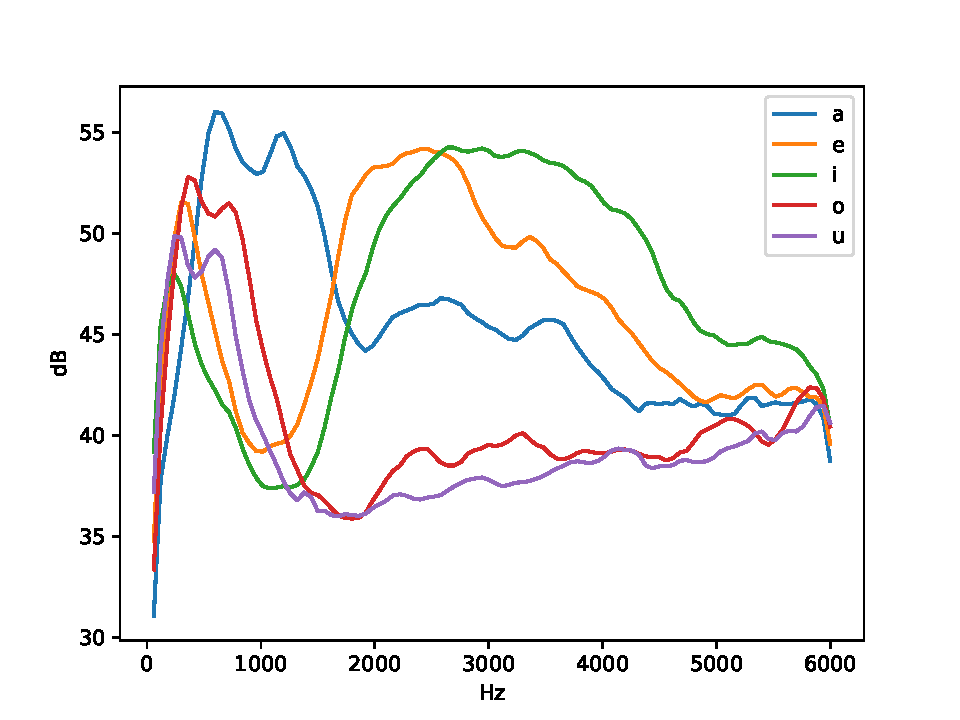
\includegraphics[scale = 0.45]{energy_distribution.pdf}
    \caption{The mean energy distribution of vowels}
    \label{fig:figenergy}
\end{figure}

\subsection{Logistic regression}

Since the clusters' centers of mass are far apart from each other, using logistic regression should produce decent results. Therefore logistic loss is an easy choice of loss function in the training phase. We will use 0/1 loss in the testing phase for logistic regression and in all the other methods we will be using.

\subsection{Decision Tree Classifier}
Since the relation between the features and labels is non-linear, it would be essential to find a non-linear model. Due to implicit performing feature selection, requiring less effort for data preparation, 
eligibility to multiple feature values, and being capable of handling categorical data, leads us to use a decision tree classifier.

\subsection{Neural Network}

The main key in using a neural network is its flexibility which can perform well for both regression and classification problems, and it is outstanding to model with non-linear data with a large number of inputs like the situation we have here. Artificial neural networks have been proven to be universal approximators, so they should work well for our problem too. We can make our dataset fit the model with a very small change: we one-hot encode the labels. We can use squared error as our loss function as it is readily implemented in the python library that we are using. In the case that our hypothesis space is a constant value, the squared error produces the average of the datapoints. Interpolating this fact to other hypothesis spaces, we see that the squared error loss produces a result that is analogous to the best average of some kind. During the evaluation phase, we can encode the results back into letters by choosing the output with the maximum value. We use $5$ hidden layers of size $20$ with the reLU function acting as our non-linearity.


\section{Results}

As we are using 0/1 - loss in the evaluation phase, we can visualize the results as nice confusion matrices. Based on the visualization of the dataset in Figure \ref{fig:figenergy}, we expect the model to clearly recognize ``a'', ``e'' and ``i'' while it is likely that ``o'' and ``u'' will get confused more often.

\subsection{Logistic Regression}

We will consider logistic regression as our baseline method. The total accuracy of this model turns out to be $85\%$ with the amplitude dataset. This is significantly higher than the result we obtain with the energy dataset, which scored $80\%$ in accuracy. As expected, the letters ``o'' and ``u'' are confused more often. Also, surprisingly ``i'' and ``e'' seem to be confused rather often, as we can see from \ref{fig:figconfusion}.

\subsection{Decision Tree Classifier}

One of the critical factors in using decision trees is the depth of the decision tree. It is known that high depth could cause overfitting in our model and make it more complex. Thus, the first step in using a decision tree is finding the best value for the depth of our decision tree to avoid underfitting and overfitting. Therefore, we used mean squared error to compute training and validation errors for decision tree regression on the amplitude dataset for the degrees of range from $1$ to $20$. We present these errors for degrees from $5$ to $10$ in Table \ref{tab:trainValErr}. It is concluded the depth of $8$ gives the minimum amount of validation error along with an acceptable amount of training error, and then, we can observe an increase in validation error indicating that the model starts to overfit. The total accuracy of this model turns out to be $84\%$ with the amplitude dataset. By doing the same approach on the energy dataset, the total accuracy of $82\%$ can be obtained which is less than the accuracy obtained from the amplitude dataset.

\begin{table}
\centering
\begin{tabular}{ |c|c|c|c|c|c|c| } 
\hline
 Degree & 5 & 6 & 7 & 8 & 9 & 10 \\  \hline
 Training Error & 0.627362 & 0.538571 & 0.401090 & 0.351654 & 0.274587  & 0.218057\\ 
 \hline
 Validation Error & 0.681900 & 0.630526 & 0.538232 & 0.534648 & 0.540621 & 0.546595 \\ 
 \hline
\end{tabular}
\caption{\label{tab:trainValErr}Training and Validation Errors for decision tree regression for degrees from 5 to 10}
\end{table}
\subsection{Neural Network}

Neural networks are somewhat similar to logistic regression in our case in the sense that the output values will be correlated to the shapes found in the input data. Therefore we expect neural networks to produce similar results to logistic regression but better since they have bluntly more predicting power. By making the hidden layers significantly smaller than the input layer we reduce the chance of overfitting. Based on Figure \ref{fig:figconfusion}, this model confuses ``o'' and ``u'' significantly less often and achieves an $88\%$ accuracy score with the amplitude dataset, and the test error obtained from this method is equal to $0.387096$ which is remarkably less than the other methods.

\subsection{Comparing methods}

Comparing the total accuracy of these three methods indicates that on a given validation set, the neural network is performing better, and confuses vowel letters less as compared to logistic regression and decision tree classifier. Thus, in this problem, neural network could be a adequate method here. Moreover, the decision tree classifier has some downsides. For instance, a small change in the data could cause a large change in the structure and shows its instability, and it also needs higher time to train the model. In the end, comparing the total accuracy and the test error indicates that the neural network is the best ML method for this problem.

\section{Conclusion}
This report represents the application of machine learning in the problem of correctly distinguishing vowels and classifying them, which can have notable use in speech recognition technology. First of all, data processing is necessary, therefore, by taking Fourier transforms and preparing the energy distribution and the amplitude distribution of samples, we start to apply machine learning methods, logistic regression, decision classifier, and neural network. In applying these methods, $20\%$ of the original set is considered as the test set and the rest is considered as the training set.

By using logistic regression, decision classifier, and neural network methods on the amplitude dataset, the total accuracy of $85\%$, $84\%$, and $88\%$ can be obtained, respectively. Besides the high accuracy obtained from the neural network, once it is trained, the prediction is pretty fast.

Even though neural network gives us the promising result for this problem, there is plenty of scope for improvement. For instance, using other machine learning methods that are robust against noisy data, might be helpful and brings us notable results. Although neural networks usually perform as well as other methods of machine learning, it requires much more data than other traditional machine learning methods. Thus, the reliability of the neural network could be enhanced with a larger dataset.

Furthermore, one of the research directions for future improvement could be considering additional features, like different accents which have effects on the amplitude distribution, we believe it would be undoubtedly beneficial to collect more data with a variety of recording environments, or even microphone positions.


\begin{figure}[!h]
    \centering
    \subfloat[Logistic Loss]{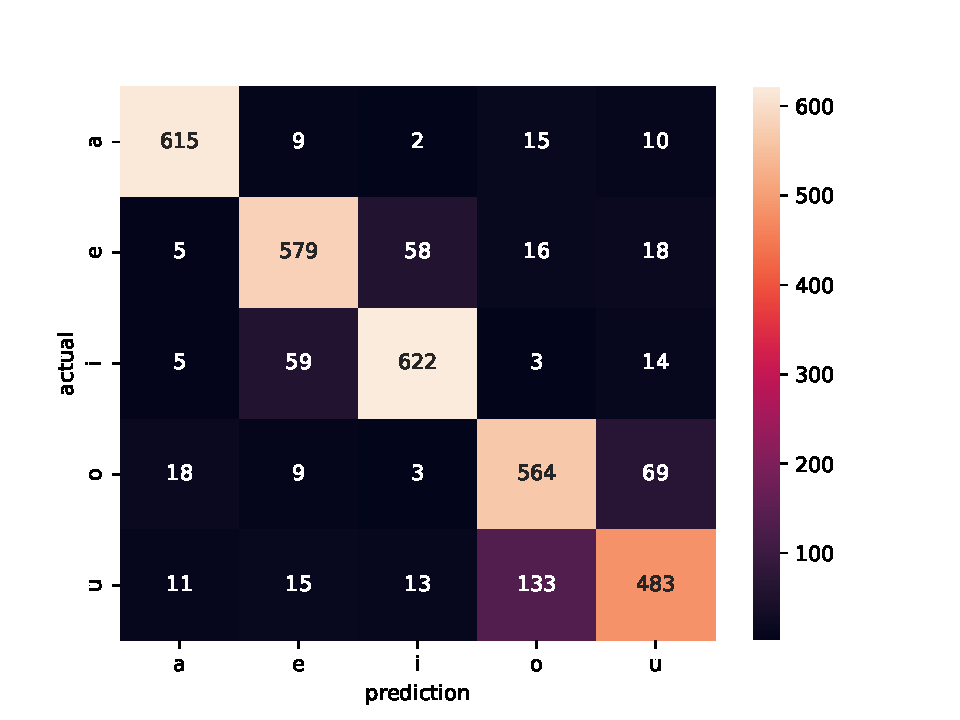
\includegraphics[scale = 0.50]{logistic_confusion.pdf}}\hfill
    \subfloat[Decision Tree Classifier]{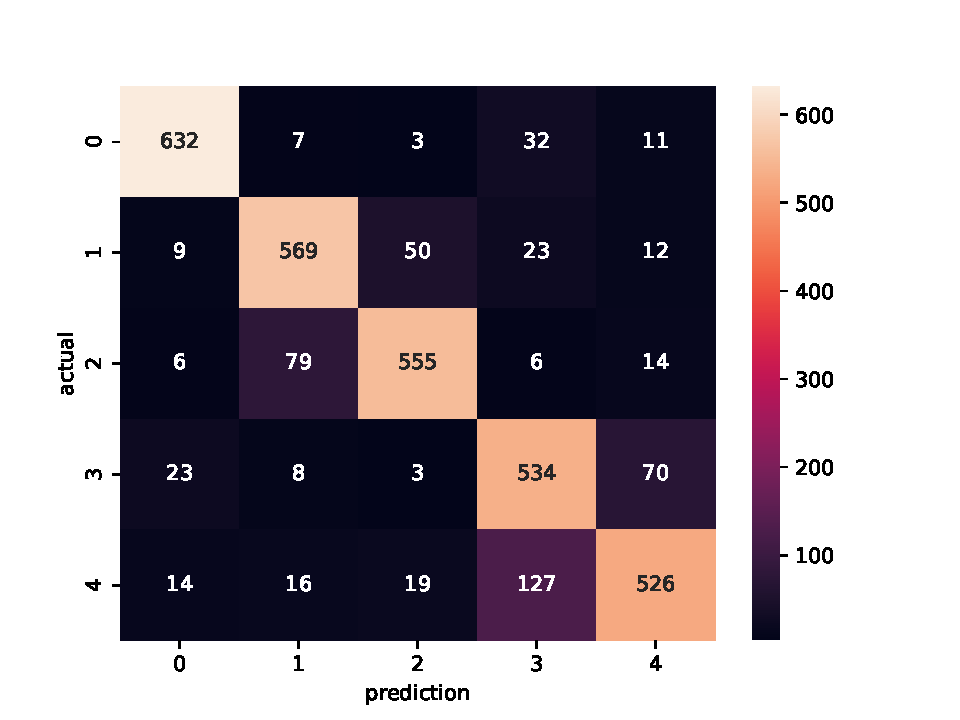
\includegraphics[scale=0.50]{decision_tree_confmat.pdf}}
    \subfloat[Neural Network]{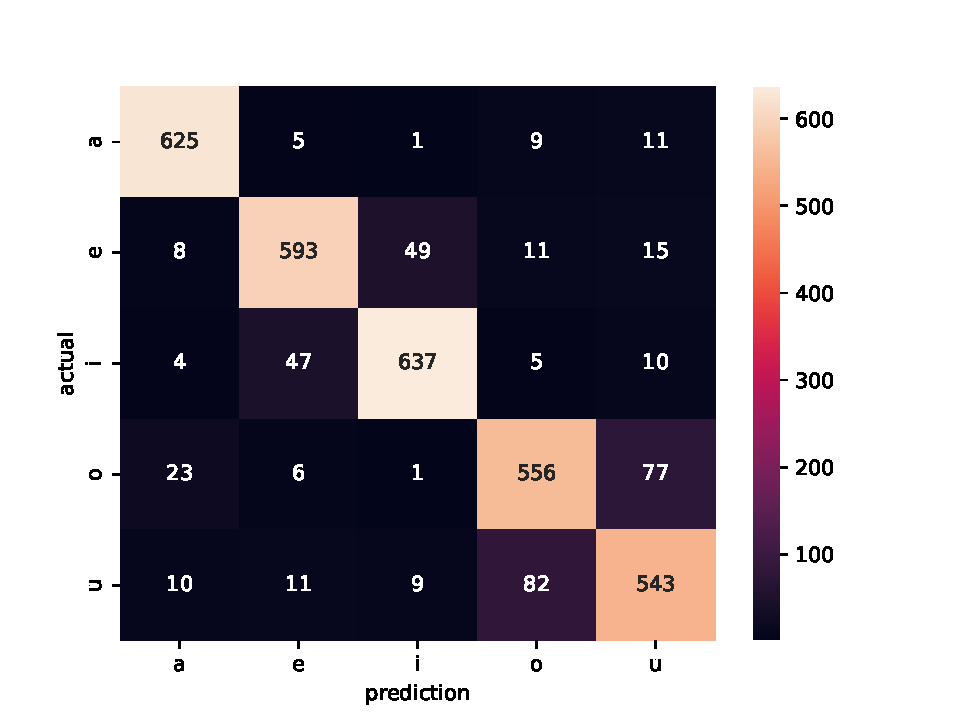
\includegraphics[scale=0.50]{NN_confusion.pdf}}
    \caption{The confusion matrices of the used ML methods.}
    \label{fig:figconfusion}
\end{figure}
\begin{thebibliography}{99}
\bibitem{dataset} DATASET\_OF\_VOWELS, available at \\ \href{https://www.kaggle.com/datasets/darubiano57/dataset-of-vowels?resource=download}{https://www.kaggle.com/datasets/darubiano57/dataset-of-vowels?resource=download}.

\bibitem{repo} Github repository, available at \\\href{https://github.com/UnilK/ML-project}{https://github.com/UnilK/ML-project}.
\end{thebibliography}

\end{document}
